\subsection{Segmentation} \label{segmenation-1}

Wie bereits in Kapitel \ref{segmentation-0} beschrieben, ist das Ziel der Segmentation Teile von Daten zu identifizieren, welche wichtige Informationen {\"u}ber die zu erkennenden Emotionen enthalten.
In dieser Projektarbeit wurde ein Schiebefensteransatz (engl. ``sliding window approach'') verwendet. 
Ziel der Methode ist die Segmentierung der vorhandenen Daten in kleinere Einheiten, um die Merkmalsextraktion sowie die anschlie{\ss}ende Klassifizierung zu vereinfachen oder gar erst zu erm{\"o}glichen.
Die L{\"a}nge des Zeitfensters (engl. ``time window'') und des Gleitschritts (engl. ``sliding stride'') sind zu bestimmende Parameter (und werden auch als ```Hyperparameter'' bezeichnet), wobei sich das Zeitfenster auf die feste Gr{\"o}{\ss}e pro extrahiertem Segment und der Gleitschritt auf den Abstand zu dem Beginn des darauf folgenden Zeitfensters bezieht.
Es ist zu beachten, dass sich aufeinanderfolgende Zeitfenster {\"u}berlappen k{\"o}nnen, sobald der definierte Gleitschritt kleiner als das Zeitfenster ist. \\


Die Daten werden auf Zeitstempel-Ebene mit Etiketten beschriftet, basierend auf den von der jeweiligen Versuchsperson ausgef{\"u}llten Frageb{\"o}gen. 
Jedem Zeitfenster wird ein Etikett zugeordnet, welches das dominate (d.h. am meisten vohandene) Etikett der im entsprechendem Fenster enthaltenen Zeitstempel basiert. Es wird davon ausgegangen, dass jedes Zeitfenster nur von einer Emotion belegt ist. \\


\begin{figure}[h]
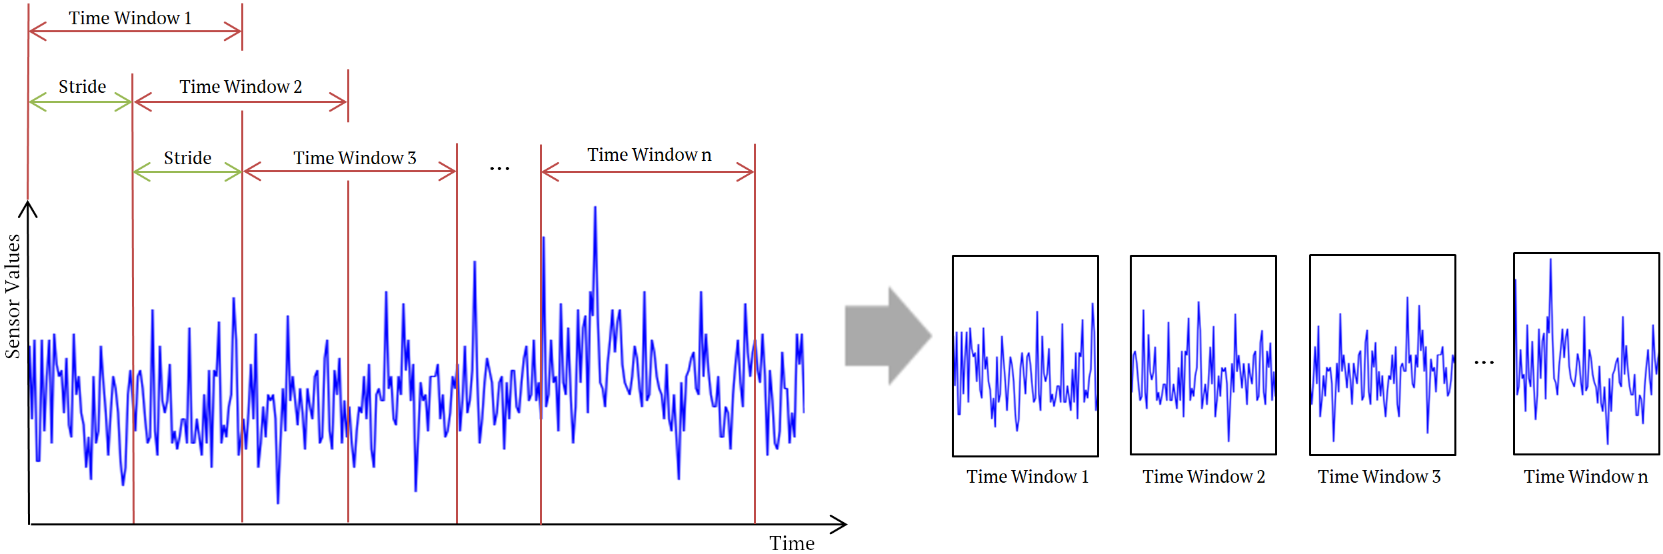
\includegraphics[width=\textwidth]{Images/segmentation.png} 
\caption[Schiebefenster-Segmentierung]{Schiebefenster-Segmentierung: Die Daten werden durch ein Zeitfenster fester Gr{\"o}{\ss}e in kleinere Segmente aufgeteilt. Das Fenster wird mit einem festen Gleichschritt geschoben, um den aufeinanderfolgend Daten-Zeitfenster zu erhalten. }
\end{figure} 